% !Mode:: "TeX:UTF-8"
%(美)C.Henry Edwards David E. Penney著,张友 王立东 袁学刚 译 清华大学出版社 ISBN: 978-7-302-14246-1
\chapter{微分方程与边值问题}
\section{一阶微分方程}
\begin{theorem}
  ({\bf 解的存在性和唯一性})假设函数$f(x,y)$和他的偏导数$\frac{\partial f}{\partial y}$, 在xy平面上含有点$(a,b)$ 的某一矩形区域上连续,那么初始问题
  \begin{equation}
    \frac{dy}{dx}=f(x,y),y(a)=b
  \end{equation}
  在含有点a 的开区间I 上有且仅有定义在区间I 上的一个解.
  \label{existence et unicite}
\end{theorem}
\begin{example}
  在微分方程$dy/dx=-y$中,函数$f(x,y)=-y$和偏导数$\frac{\partial f}{\partial y}=-1$在整个xy平面上连续,因此由定理\ref{existence et unicite} 知,对任意的初始值(a,b) 都有唯一解,尽管定理肯定了解存在于含有x=a 的某一个区间上,但是对于所有x 来讲$y(x)=Ce^{-x}$ 都被定义为解.
\end{example}
\begin{note}
  之前,我们讨论了非常简单的微分方程$\frac{dy}{dx}=y^2$, 这里$f(x,y)=y^2,\frac{\partial f}{\partial y}=2y$. 这两个函数在xy平面上都连续,特别在矩形$-2<x<2,0<y<2 $ 上也连续.由于点(0,1) 属于该矩形,所以根据定理\ref{existence et unicite}, 初值问题
  \begin{equation}
    \frac{dy}{dx}=y^2,y(0)=1
  \end{equation}
  在含有a=0的某个区间上有唯一解,确实,他就是我们之前求过的解$$y(x)=\frac{1}{1-x}$$
  但是,在x=1处,1/(1-x)不连续,所以在整个区间$-2<x<2 $上不存在唯一连续解,这样,定理\ref{existence et unicite}中的解区间I可能不像矩形$-2<x<2,0<y<2$ 那么宽,该矩形上函数 f(x,y)和偏导数$\frac{\partial f}{\partial y}$ 都连续. 从几何上讲,其原因是定理给出的解曲线在它达到区间的又给或两个端点之前,可能离开了矩形,而在矩形内部的解一定存在 \newline
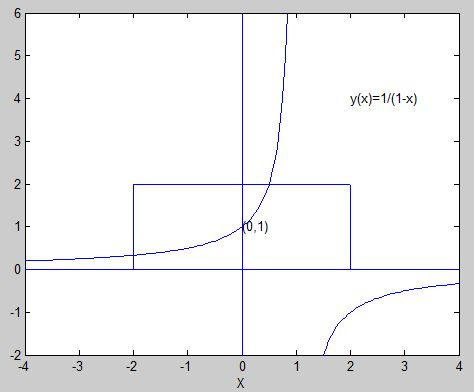
\includegraphics[width=200pt]{1-3-8}\\
图中解曲线在到达区间I的右端点之前离开矩形I
\end{note}
\subsection{一阶线性微分方程}
\begin{theorem}
  在两个系数函数P(x)与Q(x)都连续的某一区间上,求解一阶线性微分方程
  \begin{equation}
    \frac{dy}{dx}+P(x)y=Q(x)
    \label{equation 1}
  \end{equation}
  通过对\ref{equation 1}两边乘以适当的积分因子,可以得到一种标准解法,我们乘以
  \begin{equation}
   {\bf  \rho(x)=e^{\int P(x)dx}}
    \label{equation 2}
  \end{equation}
 结果为
 \begin{equation}
    e^{\int P(x)dx} \frac{dy}{dx}+P(x)e^{\int P(x)dx}y=Q(x)e^{\int P(x)dx}
    \label{equation 3}
  \end{equation}
  方程\ref{equation 3}的左边是$y(x)e^{\int P(x)dx}$的微分
  两边积分,最后求出\ref{equation 1}的通解为:
  \begin{equation}
    y(x)=e^{-\int P(x)dx}({\int {Q(x)e^{\int P(x)}dx} }+C)
  \end{equation}
\end{theorem}

\subsection{替换方法和恰当方程}
\begin{theorem}
  形如$\frac{dy}{dx}=F(ax+by+c)$ 的微分方程可以通过变换$v=ax+by+c$ 将其变化分离变量型
\end{theorem}
\subsection{恰当微分方程}
\begin{theorem}
  {\bf (恰当型判别准则)}假设在矩形开区域$R:a<x<b,c<y<d$ 上,函数M(x,y),N(x,y)连续且有连续一阶偏导数,那么微分方程
  \begin{equation}
  M(x,y)dx+N(x,y)dy=0
\end{equation}
是恰当型的充要条件是
\begin{equation}
  \frac{\partial M}{\partial y}=\frac{\partial N}{\partial x}
  \label{equation 4}
\end{equation}
在矩形R上成立.即存在R上的函数F(x,y), 满足$\frac{\partial f}{\partial x}=M,\frac{\partial f}{\partial y}=N$ 的充要条件是式\ref{equation 4}在矩形R 上成立.
\end{theorem}

\begin{note}
  一般的,为了求解恰当方程$M(x,y)dx+N(x,y)dy=0$, 我们执行以下步骤: \newline
  首先,把M(x,y) 对x 进行积分,且写成下面的形式
  $$
  F(x,y)=\int M(x,y)dx+g(y)
  $$
  然后通过$\frac{\partial F}{\partial y}=N(x,y)$ 求出g(y), 这样就得到方程的隐式解 $F(x,y)=C$
\end{note}
\begin{example}
  求解微分方程$(6xy-y^2)dx+(4y+3x^2-3xy^2)dy=0$ \newline
  解:设$M(x,y)=(6xy-y^2),N(x,y)=(4y+3x^2-3xy^2)$ 因为
  $$
  \frac{\partial M}{\partial y}=6x-3y^2=\frac{\partial N}{\partial x}
  $$
  所以方程是恰当的
  $$
  F(x,y)=\int M(x,y)dx+g(y)=\int (6xy-y^2)dx+g(y)=3x^2y-xy^3+g(y)
  $$
  然后对y进行微分,并设$\frac{\partial f}{\partial y}=N(x,y)$ 得到
  $$
  \frac{\partial f}{\partial y}=3x^2-3xy^2+g'(y)=4y+3x^2-3xy^2
  $$
  整理得到:$g'(y)=4y$, 于是$g(y)=2y^2+C_1$, 从而
  $$
  F(x,y)=3x^2y-xy^3+2y^2+C_1
  $$
  因此微分方程的隐式通解为$$3x^2y-xy^3+2y^2=C$$
\end{example}

\section{数值逼近}
\subsection{欧拉方法}
已知初值问题
\begin{equation}
  \frac{dy}{dx}=f(x,y),y(x_0)=y_0.
\end{equation}
{\bf 步长为h的欧拉方法}:应用迭代公式
\begin{equation}
  y_{n+1}=y_n+hf(x_n,y_n) ~~~(n\geqslant 0)
\end{equation}
来依次计算在各个点$x_1,x_2,x_3,\ldots,x_n$ 对真实解y=f(x)的真实值$y(x_1),y(x_2),\ldots,y(x_n)$ 的逼近值$y_1,y_2,\ldots,y_n$
\newline

\subsection{改进的欧拉方法}
已知初值问题
\begin{equation}
  \frac{dy}{dx}=f(x,y),y(x_0)=y_0.
\end{equation}
假设对步长h执行n步以后,已经得到在$x_n=x_0+nh$ 点解的真值$y(x_n)$ 逼近值$y_n$, 可应用欧拉方法来获得在点$x_{n+1}=x_n+h$ 的解的真值的一个初步估计,即称之为$u_{n+1}$ 而不是$y_{n+1}$ ,则
\begin{equation}
  u_{n+1}=y_n+hf(x_n,y_n)=y_n+hk_1. \quad k_1=f(x_n,y_n)
\end{equation}
既然$u_{n+1}\thickapprox y(x_{n+1})$, 可取$k_2=f(x_{n+1},y_{n+1})$ 作为解曲线$y=f(x)$在$x=x_{x+1}$ 点的斜率的第二个估计. \newline
当然,我们已经求出在$x=x_n$的近似斜率$k_1=f(x_n,y_n)$. 为了获得在整个区间$[x_n,x_{x+1}]$ 上解曲线平均斜率的更加精确的估计,为什么不平均这两个斜率呢? \newline 这个思想就是改进的欧拉方法的本质.
\begin{theorem}
  {\bf 算法~~~改进的欧拉方法} \newline
给定初值问题
\begin{equation}
  \frac{dy}{dx}=f(x,y),y(x_0)=y_0.
\end{equation}
步长为h的欧拉方法:应用迭代公式
$
\begin{cases}
  k_1=f(x_n,y_n) \\
  u_{n+1}=y_n+hk_1 \\
  k_2=f(x_{n+1},y_{n+1}) \\
  y_{n+1}=y_n+\frac{1}{2}h(k_1+k_2)
\end{cases}
$
\\
来依次计算$y=f(x)$在点$x_1,x_2,x_3,\ldots,x_n$的真值$y(x_1),y(x_2),\ldots,y(x_n)$ 的逼近值$y_1,y_2,\ldots,y_n$. 
\end{theorem}
\begin{note}
  改进后的欧拉方法使用的是一种称为{\bf 预测-校正}方法的一类数值技术之一. 首先计算下一个y值的预测值$u_{n+1}$ ,然后它自我校正. 这样步长为h的改进的欧拉方法\\
  由使用预测值
  \begin{equation}
    u_{n+1}=y_n+hf(x_n,y_n)
  \end{equation}
  和校正值
  \begin{equation}
    y_{n+1}=y_n+\frac{1}{2}h(f(x_n,y_n)+f(x_{n+1},y_{n+1}))
  \end{equation}
  构成.
\end{note}

\subsection{龙格-库塔方法}

